%%%%%%%%%%%%%%%%%%%%%%%%%%%%%%%%%%%%%%%%%%%%%%%%%%%%%%%%%%%%%%%%%%%%%%%%%%%%%%%
\section{Improving Robustness of Convolution Neural Networks with Doubly-Block Toeplitz matrices}
%%%%%%%%%%%%%%%%%%%%%%%%%%%%%%%%%%%%%%%%%%%%%%%%%%%%%%%%%%%%%%%%%%%%%%%%%%%%%%%

\subsection{Defending against Adversarial Attacks}

%%%%%%%%%%%%%%%%%%%%%%%%%%%%%%%%%%%%%%%%%%%%%%%%%%%%%%%%%%%%%%%%%%%%%%%%%%%%%%%
\begin{frame}{Defending against Adversarial Attacks}
%%%%%%%%%%%%%%%%%%%%%%%%%%%%%%%%%%%%%%%%%%%%%%%%%%%%%%%%%%%%%%%%%%%%%%%%%%%%%%%

  An \textbf{Adversarial Attack} aims to find the worst perturbation $\tau$ with $\norm{\tau}_p \leq \epsilon$ in such a way that the Neural Network misclassifies. Therefore, an attacker aims to find the solution to the following problem:
  \begin{equation*}
    \tau_{\theta}^{\mathrm{adv}}(\xvec) \triangleq \max_{\norm{\tau}_p \leq \epsilon} \mathcal{L}(\mathcal{N}_\theta(\xvec + \tau), y)
  \end{equation*}

  \cite{goodfellow2014explaining} have proposed \textbf{Adversarial Training} which follows \textbf{ERM} training over adversarially-perturbed samples
  \begin{equation*}
    \argmin_{\theta} \frac{1}{n} \sum_{i=1}^{n} \mathcal{L} (\mathcal{N}_\theta (\xvec_i + \tau_{\theta}^{\mathrm{adv}}(\xvec_i)), y_i)
  \end{equation*}
      
  % This algorithm consists to training the neural network on the worst case adversarial attacks instead of natural images.
  \citet{farnia2018generalizable} have shown that the adversarial generalization error depends on the Lipschitz constant of the network. 
  \begin{itemize}
    \item[$\Rightarrow$] Reducing the Lipschitz constant of the Neural Network improves the robustness against adversarial attacks.
  \end{itemize}

\end{frame}


% %%%%%%%%%%%%%%%%%%%%%%%%%%%%%%%%%%%%%%%%%%%%%%%%%%%%%%%%%%%%%%%%%%%%%%%%%%%%%%%
% \begin{frame}{Improving Robustness with Lipschitz Regularization}
% %%%%%%%%%%%%%%%%%%%%%%%%%%%%%%%%%%%%%%%%%%%%%%%%%%%%%%%%%%%%%%%%%%%%%%%%%%%%%%%
%
%   \citet{farnia2018generalizable} have shown that the adversarial generalization error depends on the Lipschitz constant of the network. 
%   \begin{itemize}
%     \item[$\Rightarrow$] Reducing the Lipschitz constant of the Neural Network will improve robustness against adversarial attacks
%   \end{itemize}
%
%   % $\Rightarrow$ Adversarial test error can be improved by reducing the Lipschitz regularization in addition to adversarial training, we propose the following:
%
% \end{frame}


%%%%%%%%%%%%%%%%%%%%%%%%%%%%%%%%%%%%%%%%%%%%%%%%%%%%%%%%%%%%%%%%%%%%%%%%%%%%%%%
\begin{frame}{Lipschitz constant of a Neural Network}
%%%%%%%%%%%%%%%%%%%%%%%%%%%%%%%%%%%%%%%%%%%%%%%%%%%%%%%%%%%%%%%%%%%%%%%%%%%%%%%
  The \textbf{Lipschitz constant} w.r.t $\ell_2$ of a function is the smallest constant K such that:
  \begin{equation*}
    \norm{f(\xvec) - f(\yvec)}_2 \leq K \norm{\xvec - \yvec}_2
  \end{equation*}
  Let us denote $\lip(f) = K$ or that $f$ is $K$-Lipschitz.

  The Lipschitz constant of the composition of multiple functions can be upper bounded by the product of the Lipschitz constant of each function.

  Remarks:
  \begin{itemize}
    \small
    \item[$\bullet$] For a linear function, the Lipschitz constant also corresponds to the maximal singular value. 
    \item[$\bullet$] Usual non-linear functions used in Neural Networks (\eg ReLU) are 1-Lipschitz
  \end{itemize}

  Therefore, we can upper bound the Lipschitz constant of a Neural Network $\mathcal{N}$ as follows:
  \begin{equation*}
    \lip(\mathcal{N}_\theta) \leq \prod_{i=0}^\ell \lip(\phi_{\Wmat_i, \bvec_i}) = \prod_{i=0}^\ell \sigma_1(\Wmat_i)
  \end{equation*}

  \begin{itemize}
    \item[$\Rightarrow$] This bound is hard to compute
  \end{itemize}
 
\end{frame}




\subsection{Bounding the singular values of Convolutional Layers}


%%%%%%%%%%%%%%%%%%%%%%%%%%%%%%%%%%%%%%%%%%%%%%%%%%%%%%%%%%%%%%%%%%%%%%%%%%%%%%%
\begin{frame}{Convolution as matrix-multiplication}
%%%%%%%%%%%%%%%%%%%%%%%%%%%%%%%%%%%%%%%%%%%%%%%%%%%%%%%%%%%%%%%%%%%%%%%%%%%%%%%

  A discrete convolution between a signal $\xvec$ and a kernel $\kvec$ can be expressed as a product between the vectorization of $\xvec$ and a doubly-block Toeplitz matrix $\Mmat$, whose coefficients have been chosen to match the convolution $\xvec * \kvec$.

  \begin{figure}
    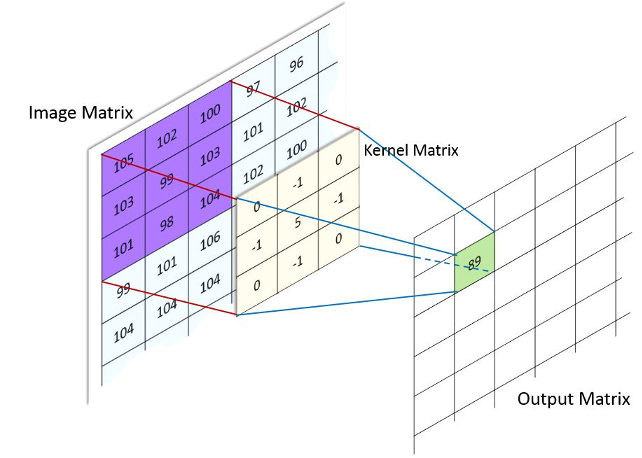
\includegraphics[width=0.5\textwidth]{images/convolution.png}
    \caption*{Convolution between a 2-dimensional image and a 2 dimensional kernel}
  \end{figure}

  The convolution is equivalent to a matrix-vector product between a \textbf{doubly-block Toeplitz matrix} and the vectorize image. 

\end{frame}


%%%%%%%%%%%%%%%%%%%%%%%%%%%%%%%%%%%%%%%%%%%%%%%%%%%%%%%%%%%%%%%%%%%%%%%%%%%%%%%
\begin{frame}{Convolution as matrix-multiplication}
%%%%%%%%%%%%%%%%%%%%%%%%%%%%%%%%%%%%%%%%%%%%%%%%%%%%%%%%%%%%%%%%%%%%%%%%%%%%%%%


  In practice, the image has multiple \textbf{channels} (\eg RGB). We refer to the number of input channels $cin$ and the number of output channels $cout$.

  \begin{figure}
    \begin{subfigure}[t]{0.49\textwidth}
      \centering
      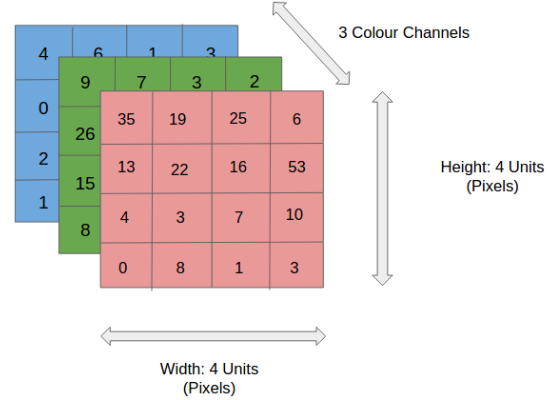
\includegraphics[width=0.8\textwidth]{images/image_rgb.png}
      \caption*{}
    \end{subfigure}
    \begin{subfigure}[t]{0.45\textwidth}
      \centering
      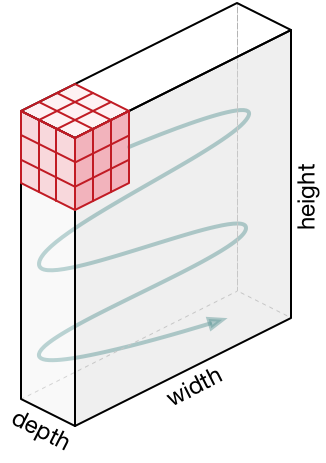
\includegraphics[width=0.5\textwidth]{images/conv_2d.png}
      \caption*{}
    \end{subfigure}
  \end{figure}

  A multi-channel convolution is equivalent to a matrix-vector product where the matrix is a \textbf{block matrix} where each block is doubly-block Toeplitz matrix. 

\end{frame}



%%%%%%%%%%%%%%%%%%%%%%%%%%%%%%%%%%%%%%%%%%%%%%%%%%%%%%%%%%%%%%%%%%%%%%%%%%%%%%%
\begin{frame}{Generating functions of Toeplitz and block Toeplitz matrices}
%%%%%%%%%%%%%%%%%%%%%%%%%%%%%%%%%%%%%%%%%%%%%%%%%%%%%%%%%%%%%%%%%%%%%%%%%%%%%%%
    
  A $n\times n$ Toeplitz matrix $\Amat$ is fully determined by a two-sided sequence of scalars: $\{a_\seqidx\}_{\seqidx \in \seqsetN}$, whereas a $nm \times nm$ block Toeplitz matrix $\Bmat$ is fully determined by a two-sided sequence of blocks $\{\Bmat_\seqidx\}_{\seqidx \in \seqsetN}$, where $\seqsetN = \{-n+1,\dots, n-1 \}$ and where each block $\Bmat_\seqidx$ is a $m \times m$ matrix.  

  \begin{equation*}
      \Amat = \begin{pmatrix}
	a_0 & a_{1} & \cdots & a_{n-1} \\ \vspace{0.1cm}
	a_{-1} & a_0 & \ddots & \vdots \\ \vspace{0.3cm}
       \vdots & \ddots & a_{0} & a_{1} \\ 
      a_{-n+1} & \cdots  & a_{-1}    & a_0 
      \end{pmatrix} \quad \quad \quad \quad 
      \Bmat =\begin{pmatrix}
	\Bmat_0 & \Bmat_{1} & \cdots & \Bmat_{n-1} \\ \vspace{0.1cm}
	\Bmat_{-1} & \Bmat_0 & \ddots & \vdots \\ \vspace{0.3cm}
       \vdots & \ddots & \Bmat_0 & \Bmat_{1} \\ 
      \Bmat_{-n+1} & \cdots  & \Bmat_{-1}    & \Bmat_0 
      \end{pmatrix}.
  \end{equation*}

  We also write:
  \begin{equation*}
    \Amat = (a_{j-i})_{i, j \in \{0, \dots, n-1\}} \quad \quad
    \Bmat = (\Bmat_{j-i})_{i, j \in \{0, \dots, n-1\}}
  \end{equation*}

\end{frame}


%%%%%%%%%%%%%%%%%%%%%%%%%%%%%%%%%%%%%%%%%%%%%%%%%%%%%%%%%%%%%%%%%%%%%%%%%%%%%%%
\begin{frame}{Generating functions of Toeplitz and block Toeplitz matrices}
%%%%%%%%%%%%%%%%%%%%%%%%%%%%%%%%%%%%%%%%%%%%%%%%%%%%%%%%%%%%%%%%%%%%%%%%%%%%%%%

  % A standard tool for manipulating (block) Toeplitz matrices is the use of Fourier analysis.

  Let us define a complex-valued function and a matrix-valued function which are the \emph{inverse Fourier Transform} of the sequences $\{a_h\}_{h \in N}$ and $\{\Bmat\}_{h \in N}$ as follows:
  \begin{equation*}
    f(\omega) = \sum_{h \in N} a_h e^{\ci h \omega} \quad \quad F(\omega) = \sum_{h \in N} \Bmat_h e^{\ci h \omega} 
  \end{equation*}

  % Theses functions are the \emph{inverse Fourier Transform} of the sequences $\{a_h\}_{h \in N}$ and $\{\Bmat\}_{h \in N}$.  
  One can recover these two sequences using the standard Fourier transform:

  \begin{equation*}
    a_\seqidx = \frac{1}{2\pi} \int_0^{2\pi} e^{-\ci \seqidx \omega} f(\omega) d\omega \quad \quad \Bmat_\seqidx = \frac{1}{2\pi} \int_0^{2\pi} e^{-\ci \seqidx \omega} F(\omega) d\omega .
  \end{equation*}

  From there, we can define an operator $\Tmat$ mapping integrable $2\pi$-periodic functions to Toeplitz or block Toeplitz matrices:
  \begin{equation*}
    \Tmat(g) \triangleq\leftmat\frac{1}{2\pi}\int_{0}^{2\pi}e^{-\ci(i-j)\omega}g(\omega)\,d\omega\rightmat_{i,j\in\{0,\ldots,n-1\}} . 
  \end{equation*}

  % This operator has been extensively studied by~\citet{gray2006toeplitz} and~\citet{gutierrez2012block}

\end{frame}



%%%%%%%%%%%%%%%%%%%%%%%%%%%%%%%%%%%%%%%%%%%%%%%%%%%%%%%%%%%%%%%%%%%%%%%%%%%%%%%
\begin{frame}{Operator for Doubly-Block Toeplitz matrices}
%%%%%%%%%%%%%%%%%%%%%%%%%%%%%%%%%%%%%%%%%%%%%%%%%%%%%%%%%%%%%%%%%%%%%%%%%%%%%%%

  Because doubly-block Toeplitz matrices are \textbf{block Toeplitz} where each block is a \textbf{Toeplitz matrix}, we can extend the reasoning with a 2 dimensional function  $f: \Rbb^2 \rightarrow \Cbb$.
  
  The block Toeplitz can be written as follows:
  \begin{equation*}
    \Dmat(f) =\leftmat\Dmat_{i,j}(f)\rightmat_{i,j\in\{0,\ldots ,n-1\}}
  \end{equation*}
  and each block $\Dmat_{i,j}$ is defined as:
  \begin{equation*}
    \Dmat_{i,j}(f) =\leftmat\frac{1}{4\pi^{2}}\int_{[0,2\pi]^{2}}e^{-\mathbf{i}\left((i-j)\omega_{1}+(k-l)\omega_{2}\right)}f(\omega_{1},\omega_{2})\,d(\omega_{1},\omega_{2})\rightmat_{k,l\in\{0,\ldots,m-1\}} .
  \end{equation*}

  The operator $\Dmat$ which maps a function $f: \Rbb^2 \rightarrow \Cbb$ to a doubly-block Toeplitz matrix of size $nm \times nm$.

\end{frame}


%%%%%%%%%%%%%%%%%%%%%%%%%%%%%%%%%%%%%%%%%%%%%%%%%%%%%%%%%%%%%%%%%%%%%%%%%%%%%%%
\begin{frame}{Bound on the singular value of Doubly-Block Toeplitz matrices}
%%%%%%%%%%%%%%%%%%%%%%%%%%%%%%%%%%%%%%%%%%%%%%%%%%%%%%%%%%%%%%%%%%%%%%%%%%%%%%%

  \begin{theorem}[Bound on the maximal singular value of a Doubly-Block Toeplitz Matrix]
    Let $\Dmat (f) \in \Rbb^{nm \times nm}$ be a doubly-block Toeplitz matrix generated by the function $f$, then:
    \begin{equation*}
      \sigma_1 \left( \Dmat(f) \right) \leq \sup_{\omega_1, \omega_2 \in [0, 2\pi]^2} |f(\omega_1,\omega_2)|
    \end{equation*}
    where the function $f: \Rbb^2 \rightarrow \Cbb$, is a multivariate trigonometric polynomial of the form:
    \begin{equation*}
      f(\omega_1, \omega_2) \triangleq \sum_{h_1 \in \seqsetN} \sum_{h_2 \in \seqsetM} d_{h_1, h_2} e^{\ci (h_1 \omega_1 + h_2 \omega_2)},
    \end{equation*}
    where $d_{h_1, h_2}$ is the ${h_2}^\mathrm{th}$ scalar of the ${h_1}^\mathrm{th}$ block of the doubly-Toeplitz matrix $\Dmat(f)$, and where $\seqsetM = \{-m+1,\dots, m-1 \}$.
  \end{theorem}

\end{frame}


% %%%%%%%%%%%%%%%%%%%%%%%%%%%%%%%%%%%%%%%%%%%%%%%%%%%%%%%%%%%%%%%%%%%%%%%%%%%%%%%
% \begin{frame}{Bound Singular Values of Convolution}
% %%%%%%%%%%%%%%%%%%%%%%%%%%%%%%%%%%%%%%%%%%%%%%%%%%%%%%%%%%%%%%%%%%%%%%%%%%%%%%%
%
%   \begin{theorem}[Bound on the maximal singular value of stacked Doubly-block Toeplitz matrices]
%       Consider doubly-block Toeplitz matrices $\Dmat(f_1), \dots, \Dmat(f_{\cin})$ where $f_i: \Rbb^2 \rightarrow \Cbb$ is a generating function. Construct a matrix $\Mmat$ with $\cin\times n^2$ rows and $n^2$ columns, as follows:
%       \begin{equation*}
% 	  \Mmat \triangleq \leftmat \Dmat^\top(f_1), \dots, \Dmat^\top(f_{\cin}) \rightmat^\top .
%       \end{equation*}
%       Then, with $f_i$ a multivariate polynomial, we have:
%       \begin{equation*} 
%          \sigma_1\left(\Mmat \right) \leq \sup_{\omega_1, \omega_2 \in \left[0, 2\pi\right]^2} \sqrt{ \sum_{i=1}^{\cin} \left|f_i\right (\omega_1, \omega_2)|^2} .
%       \end{equation*}
%     \end{theorem}
%
% \end{frame}


%%%%%%%%%%%%%%%%%%%%%%%%%%%%%%%%%%%%%%%%%%%%%%%%%%%%%%%%%%%%%%%%%%%%%%%%%%%%%%%
\begin{frame}{Bound Singular Values of Convolution}
%%%%%%%%%%%%%%%%%%%%%%%%%%%%%%%%%%%%%%%%%%%%%%%%%%%%%%%%%%%%%%%%%%%%%%%%%%%%%%%

  \begin{theorem}[Bound on the maximal singular value on the convolution operation]
    Let us define doubly-block Toeplitz matrices $\Dmat(f_{11}), \dots, \Dmat(f_{\cin\times \cout})$ where $f_{ij}: \Rbb^2 \rightarrow \Cbb$ is a generating function. Construct a matrix $\Mmat$ with $\cin\times n^2$ rows and $\cout\times n^2$ columns such as
    {\small
    \begin{equation*}
	\Mmat \triangleq  \leftmat\begin{array}{ccc}
	\Dmat(f_{11}) & \cdots & \Dmat(f_{1,\cout})   \\
	\vdots & & \vdots   \\
	\Dmat(f_{\cin,1}) & \cdots & \Dmat(f_{\cin,\cout}) \\
	\end{array}\rightmat .
    \end{equation*}
    }
    Then, with $f_{ij}$ a multivariate polynomial, we have:
    \begin{equation*}
       \sigma_1(\Mmat) \leq \sqrt{ \sum_{i=1}^{\cout} \sup_{\omega_1, \omega_2 \in [0, 2\pi]^2} \sum_{j = 1}^{\cin} \left|f_{ij}(\omega_1, \omega_2) \right|^2 } .
    \end{equation*}
  \end{theorem}

  In the following, for a given convolution layer parametrized by $\Wmat$, we will call this bound $\lipbound(\Wmat)$

\end{frame}



%%%%%%%%%%%%%%%%%%%%%%%%%%%%%%%%%%%%%%%%%%%%%%%%%%%%%%%%%%%%%%%%%%%%%%%%%%%%%%%
\subsection{Experiments}
%%%%%%%%%%%%%%%%%%%%%%%%%%%%%%%%%%%%%%%%%%%%%%%%%%%%%%%%%%%%%%%%%%%%%%%%%%%%%%%



%%%%%%%%%%%%%%%%%%%%%%%%%%%%%%%%%%%%%%%%%%%%%%%%%%%%%%%%%%%%%%%%%%%%%%%%%%%%%%%
\begin{frame}{Lipschitz Regularization of Convolutional Neural Networks}
%%%%%%%%%%%%%%%%%%%%%%%%%%%%%%%%%%%%%%%%%%%%%%%%%%%%%%%%%%%%%%%%%%%%%%%%%%%%%%%

  To improve the robustness of Neural Networks, we propose the following objective function:

  \begin{equation*}
    \argmin_{\theta} \frac{1}{n} \sum_{i=1}^{n} \mathcal{L} (\mathcal{N}_\theta (\xvec_i + \tau_{\theta}^{\mathrm{adv}}(\xvec_i)), y_i) + \lambda \sum_{j=0}^\ell \log(\lipbound(\Wmat_j)) 
  \end{equation*}
  where $\lambda$ is  used-defined parameter which controls the regularization.

  % The bound has been known to overestimate the real Lipschitz constant of a composition of functions. 
  % Nevertheless, we will show empirically that we can increase the robustness with this objective function
\end{frame}




%%%%%%%%%%%%%%%%%%%%%%%%%%%%%%%%%%%%%%%%%%%%%%%%%%%%%%%%%%%%%%%%%%%%%%%%%%%%%%%
\begin{frame}{Computing the bound}
%%%%%%%%%%%%%%%%%%%%%%%%%%%%%%%%%%%%%%%%%%%%%%%%%%%%%%%%%%%%%%%%%%%%%%%%%%%%%%%

  \begin{figure}[ht]
    \centering
    \begin{minipage}{.22\linewidth}
      \centering
      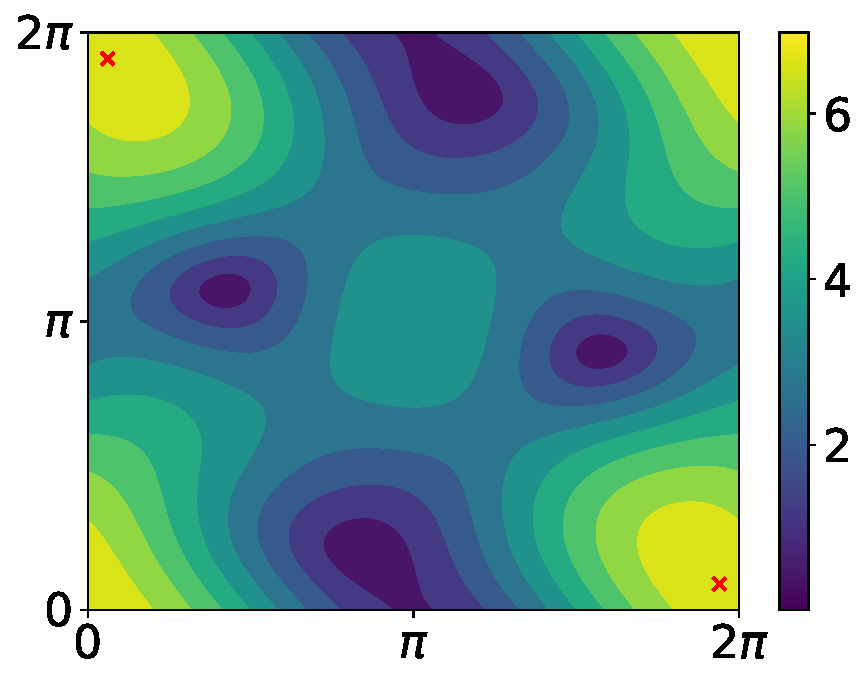
\includegraphics[scale=0.16]{images/contour_poly_200_1_1_3.pdf} \\ {\small kernel $1\times3\times3$}
    \end{minipage}
    \begin{minipage}{.22\linewidth}
	\centering
	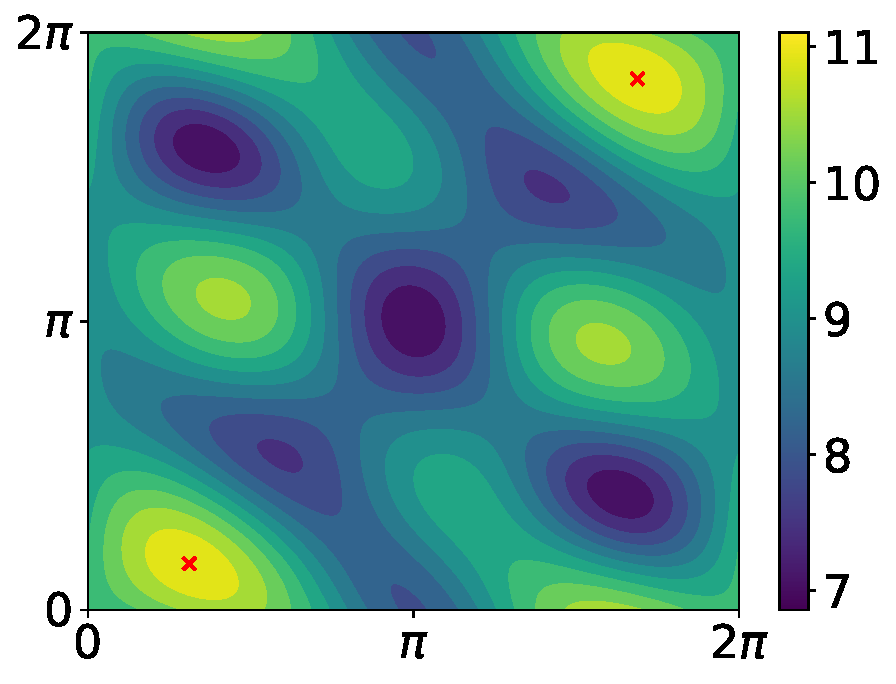
\includegraphics[scale=0.16]{images/contour_poly_200_1_9_3.pdf} \\ {\small kernel $9\times3\times3$}
    \end{minipage}
    \begin{minipage}{.22\linewidth}
	\centering
	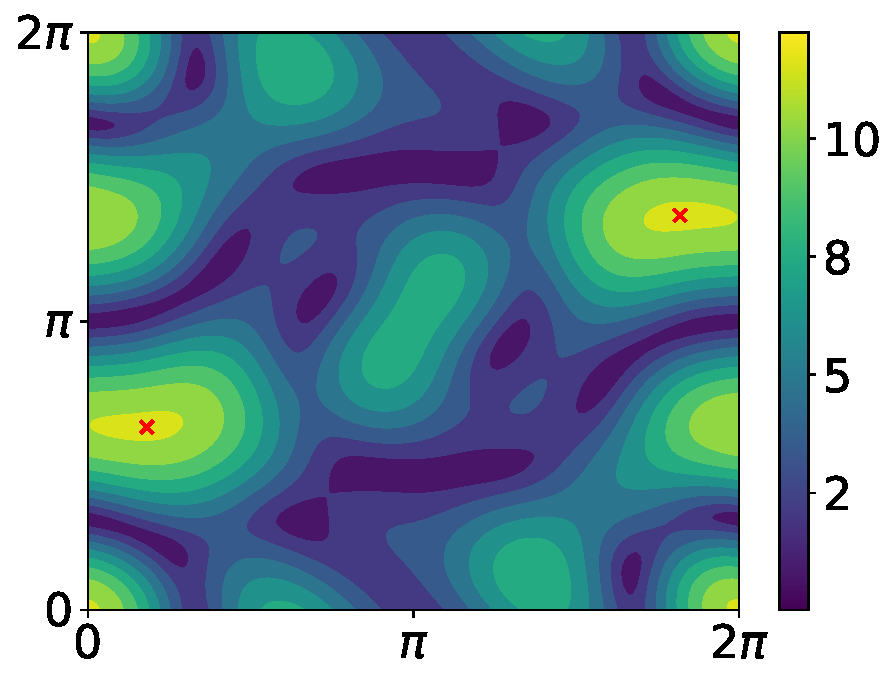
\includegraphics[scale=0.16]{images/contour_poly_200_1_1_5.pdf} \\ {\small kernel $1\times5\times5$}
    \end{minipage}
    \begin{minipage}{.22\linewidth}
	\centering
	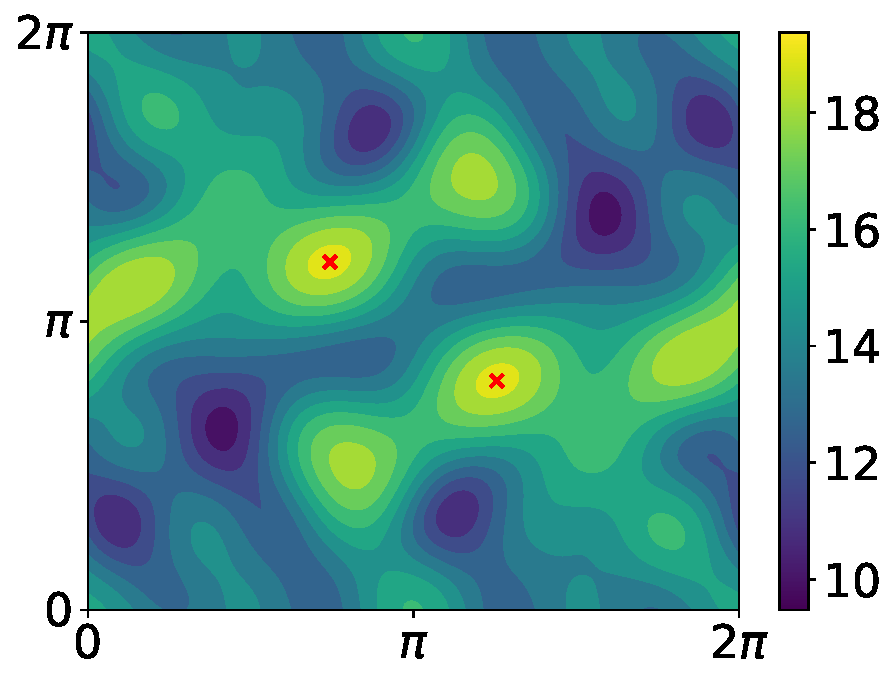
\includegraphics[scale=0.16]{images/contour_poly_200_1_9_5.pdf} \\ {\small kernel $9\times5\times5$}
    \end{minipage}
    \caption{Contour plot of multivariate trigonometric polynomials.}
    \label{fig:contour_plot_trigonometric_polynomials}
  \end{figure}%

  Computing $\lipbound$ implies to compute the maximum modulus of a 2-dimensional trigonometric polynomial on 
  $[ 0, 2\pi]^2$.

  \begin{itemize}
    \item[$\bullet$] This problem has been known to be NP-hard (\cite{pfister2018bounding})
    \item[$\bullet$] However, trigonometric polynomials defined by usual convolutional kernels have a low degree (between 1 and 3)
    \item[$\bullet$] A simple grid search algorithm is efficient and can be implemented on GPU
  \end{itemize}

\end{frame}




%%%%%%%%%%%%%%%%%%%%%%%%%%%%%%%%%%%%%%%%%%%%%%%%%%%%%%%%%%%%%%%%%%%%%%%%%%%%%%%
\begin{frame}{Empirical Results -- CIFAR-10 Dataset}
%%%%%%%%%%%%%%%%%%%%%%%%%%%%%%%%%%%%%%%%%%%%%%%%%%%%%%%%%%%%%%%%%%%%%%%%%%%%%%%

  \begin{block}{Dataset: CIFAR-10}
  \begin{itemize}
    \item 50K images
    \item 10 classes
  \end{itemize}
  \end{block}

  \begin{table}[t]
    \centering
      {\small
      \begin{tabular}{lrrrr}
      \toprule
      & \textbf{Accuracy} & \textbf{PGD-$\ell_\infty$ 0.03} & \textbf{C\&W-$\ell_2$ 0.6} & \textbf{C\&W-$\ell_2$ 0.8} \\
      \midrule
      \textbf{Baseline} & $\mathbf{0.953}$ & $\phantom{.}0.000$ & $\phantom{.}0.002$ & $\phantom{.}0.000$ \\
      \textbf{AT} & $\phantom{.}0.864$ & $\phantom{.}0.426$ & $\phantom{.}0.477$ & $\phantom{.}0.334$ \\
      \textbf{AT+LipReg} & $\phantom{.}0.808$ & $\mathbf{0.457}$ & $\mathbf{0.547}$ & $\mathbf{0.438}$ \\
      \midrule
      \textbf{Diff} & $-0.056$ & $+0.031$ & $+0.07$ & $+0.104$ \\
      \bottomrule
      \end{tabular}%
      }
    \caption{This table shows the Accuracy under $\ell_2$ and $\ell_\infty$ attacks of CIFAR10 dataset. We use $\lambda$ equals to $0.008$.}
    \label{tab:table_cifar10_robustness}%
  \end{table}%



\end{frame}





% %%%%%%%%%%%%%%%%%%%%%%%%%%%%%%%%%%%%%%%%%%%%%%%%%%%%%%%%%%%%%%%%%%%%%%%%%%%%%%%
% \begin{frame}{Empirical Results -- ImageNet Dataset}
% %%%%%%%%%%%%%%%%%%%%%%%%%%%%%%%%%%%%%%%%%%%%%%%%%%%%%%%%%%%%%%%%%%%%%%%%%%%%%%%
%
%   \begin{block}{Dataset: ImageNet}
%   \begin{itemize}
%     \item 1,2 millions images
%     \item 1000 classes
%   \end{itemize}
%   \end{block}
%
% \begin{table}[htbp]
%   \centering
%    \begin{tabular}{lrrrr}
%    \toprule
%      & \multicolumn{1}{l}{\textbf{Accuracy}} & \multicolumn{1}{c}{\textbf{PGD-}$\ell_\infty$ 0.02} & \multicolumn{1}{l}{\textbf{C\&W-}$\ell_2$ 1} & \multicolumn{1}{l}{\textbf{C\&W-}$\ell_2$ 2} \\
%    \midrule
%    AT & 0.509 & 0.251 & 0.307 & 0.168 \\
%    AT+LipReg & \textbf{0.519} & \textbf{0.259} & \textbf{0.338} & \textbf{0.204} \\
%    \bottomrule
%    \end{tabular}%
%    \caption{This table shows the accuracy and accuracy under attack of ImageNet dataset with different training schemes. We compare Adversarial Training with the combination of Lipschitz regularization and Adversarial Training (\cite{madry2018towards}). We use $\lambda$  equal to $0.01$}
% \end{table}%
%
%
% \end{frame}





